\documentclass[]{article}

%%%<
\usepackage{verbatim}
%%%>

\begin{comment}
:Title: HeLiOs logo
Based on periodic-table-of-chemical-elements.tex by Ivan Griffin
Thomas Knudsen, 2013-10-26
\end{comment}
\usepackage{helvet,graphicx}
\usepackage[paperwidth=32mm, paperheight=13.8mm, margin=0.8mm]{geometry}
\usepackage{tikz}
\usetikzlibrary{shapes,calc}
%\usepackage{sansmath}
\pagecolor{lightgray}
\begin{document}


\newcommand{\CommonElementTextFormat}[4]{
  \begin{minipage}{17mm}
    \centering
     \null$^{\raisebox{2mm}{\textsf{#2}}}_{\textsf{#1}}$ \textbf{\LARGE #3}\phantom{I}
      %\linebreak \linebreak
      %{{#4}}
  \end{minipage}
}

\newcommand{\NaturalElementTextFormat}[4]
{
  \CommonElementTextFormat{#1}{#2}{{#3}}{#4}
}

%\sansmath
\centering
\noindent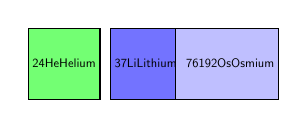
\begin{tikzpicture}[font=\sffamily, scale=0.45, transform shape]
%% Fill Color Styles
  \tikzstyle{ElementFill} = [fill=yellow!15]
  \tikzstyle{AlkaliMetalFill} = [fill=blue!55]
  \tikzstyle{AlkalineEarthMetalFill} = [fill=blue!40]
  \tikzstyle{MetalFill} = [fill=blue!25]
  \tikzstyle{MetalloidFill} = [fill=orange!25]
  \tikzstyle{NonmetalFill} = [fill=green!25]
  \tikzstyle{HalogenFill} = [fill=green!40]
  \tikzstyle{NobleGasFill} = [fill=green!55]
  \tikzstyle{LanthanideActinideFill} = [fill=purple!25]

%% Element Styles
  \tikzstyle{Element} = [draw=black, ElementFill,
    minimum width=20mm, minimum height=20mm, node distance=23mm]
  \tikzstyle{AlkaliMetal} = [Element, AlkaliMetalFill]
%  \tikzstyle{AlkalineEarthMetal} = [Element, AlkalineEarthMetalFill]
  \tikzstyle{Metal} = [Element, MetalFill]
%  \tikzstyle{Metalloid} = [Element, MetalloidFill]
%  \tikzstyle{Nonmetal} = [Element, NonmetalFill]
%  \tikzstyle{Halogen} = [Element, HalogenFill]
  \tikzstyle{NobleGas} = [Element, NobleGasFill]
%  \tikzstyle{LanthanideActinide} = [Element, LanthanideActinideFill]
%  \tikzstyle{PeriodLabel} = [font={\sffamily\LARGE}, node distance=2.0cm]
%  \tikzstyle{GroupLabel} = [font={\sffamily\LARGE}, minimum width=2.75cm, node distance=2.0cm]
%  \tikzstyle{TitleLabel} = [font={\sffamily\Huge\bfseries}]

  \node[name=He,              NobleGas] {\NaturalElementTextFormat{2}{4}{He}{Helium}};
  \node[name=Li, right of=He, AlkaliMetal] {\NaturalElementTextFormat{3}{7}{Li}{Lithium}};
  \node[name=Os, right of=Li, Metal] {\NaturalElementTextFormat{\phantom{2}76}{192}{Os}{Osmium}};
\end{tikzpicture}\\[-1.5mm]
\scalebox{0.625}{\textsf{\textbf{\textcolor{red}{He}ader \textcolor{red}{Li}braries \textcolor{red}{o}n \textcolor{red}{S}teroids}}}
\end{document}
